\chapter{Computer Vision}
\label{ComputerVision}
Computer vision is a subfield of artificial intelligence, and it aims to equip machines with the ability to perform visual tasks of recognizing and processing image data \cite{computerVisionIBM}. To us humans, this is something we don't even think about. However, the process of recognizing objects based on their geometry, color, and size is more complicated than we might think. In recent years, this field has become rather popular even outside of academic grounds, mostly thanks to autonomous cars, personal AI assistants, or even in the medical field \cite{computerVisionNX}.

% ===========================================================================================

% ===========================================================================================

\section{Object recognition as a subfield of computer vision}
As the research continued, the field widened, and so did the different techniques of computer vision, all in pursuit of general \textbf{object recognition} \cite{computerVisionIBM}.

\textbf{Image classification} is the simplest form of the object recognition task, which is the goal of computer vision. It classifies the image as a whole into predefined classes and gives it the most probable label.

\textbf{Object detection} is a further expansion of image classification; it combines object localization and image classification into one. It results in a list of coordinates or regions, along with the confidence score for these objects. These coordinates are usually in the form of rectangles and contain x and y coordinates along with the width and height. These so called bounding boxes represent detected objects in the image.

\textbf{Image segmentation} extends object detection by operating at the pixel level. Instead of predicting bounding boxes, it performs pixel-wise classification, producing masks corresponding to individual classes.

% ===========================================================================================

% ===========================================================================================

\section{Convolutional neural networks and transformer based models}

Computer vision as a research field started in the last century. As stated in \cite{computerVisionNX}, one of the first articles was released in 1943~\cite{mcculloch1943logical}, in which the researchers attempted to model artificial neurons based on biological ones. This laid the groundwork for the neural networks as we know them today. The next great leap was achieved in 2001 by Viola~\cite{viola}, who introduced a rapid object detection system capable of detecting facial features in real-time. A decade later, in 2012, Krizhevsky~\cite{krizhevsky} made another significant leap by training a deep convolutional neural network on a large dataset containing 1.2 million image samples and winning an ImageNet LSVRC-2010 contest. This changed computer vision and shifted towards using \textbf{convolutional neural networks} (hereinafter referred to as CNN) instead of traditional computer vision techniques with handcrafted feature extraction. 

A more recent trend uses \textbf{Foundation models} built utilizing \textbf{Transformer} architecture instead of CNN. Foundation models are trained on large scale datasets, often using self-supervised learning, which allows them to learn general representations from data. This allows them to be tailored to specific tasks such as object recognition. The \textbf{Transformer} architecture, often used by these models, was proposed by Vaswani in 2017~\cite{vaswani2017attention}. This approach enabled new methods for performing object recognition tasks, such as Segment Anything Models (SAM3) and Distillation of knowledge with No labels v2 (DINOv2).

% ===========================================================================================

% ===========================================================================================

\section{Object detection on edge devices}
Mobile devices, often referred to as edge devices in computer vision, still lack the raw computational power compared to the most powerful GPUs available for personal use or data centers. Even though edge devices are not the most powerful, the convenience of a computer vision capable device right in our pockets seems to be desired. This trend can be further observed, as some state-of-the-art models are being scaled down to fit into edge devices, such as EfficientSAM3~\cite{zeng2025efficientsam3}, a version of SAM3 for edge devices. This rising demand for onboard processing for low-power devices resulted in the creation of a contest named the Low-Power Image Recognition Challenge (LPIRC), which was first held in 2015~\cite{alyamkin2019low}.

This further confirmed that it is necessary to choose an architecture providing the best performance while achieving the best possible precision. A recent study shows transformer based architectures are catching up to CNNs~\cite{wang2026evolution}. However, due to its more mature architecture and better performance results, a CNN based architecture called You Only Look Once (YOLO) was chosen for this thesis. Similar results can be observed in older surveys comparing CNN architectures~\cite{objectDetectionSurvey2024, objectDetectionSurvey2025}.

\subsection{YOLO -- You Only Look Once}
\label{yolo}
In 2016, a Redmon presented a new single shot architecture called You Only Look Once~\cite{Redmon_2016_CVPR}. Other approaches, like R-CNN introduced in 2014~\cite{girshick2014rich}, search the image for possible bounding boxes and then run classifiers on those parts of the image. These are also called two stage classifiers. YOLO uses a single CNN, predicting both bounding boxes and confidence scores in one step. This approach makes YOLO fast in comparison with, up to that point in time, state-of-the art two stage CNNs. It also provides more context, as the model sees the image as a whole, unlike R-CNN, which uses a sliding window, which results in networks lacking context about the entire image.

% ===========================================================================================

% ===========================================================================================

\section{Transfer learning and pretrained models}
\label{pretrainedModels}
\label{transferLearning}
Neural networks are composed of layers. These layers are made of neurons with different weights assigned to them. The optimization of weights via backpropagation in neurons is what we call training in computer vision. Training neural networks changes their \textit{"response"} to input data (in this case, image data). This process results in neural networks progressively learning how to recognize features, which leads to the capability to detect objects.

Layers of neural networks can be grouped or separated into parts. Using YOLOv8 as an example, it is made up of a \textbf{backbone} and a \textbf{head}. Freezing the backbone part of the network and retraining the head for a specific task is called \textbf{transfer learning}. 

A very simplified example of this would be using a neural network that can distinguish geometric objects and retrain it to detect composite objects, such as eyeglasses composed of two circles and a connecting line. In this case, the first neural network, used as a backbone, understands what circles are but does not understand the concept of glasses. The newly trained head utilizes the knowledge from the backbone and learns to recognize the glasses.

Pandilova, in 2024~\cite{pandilova2024transfer}, demonstrated the use of this technique to boost the performance of the YOLOv8 object detection model. The study demonstrates that using the pretrained backbone of YOLOv8 and training it for a specific task gave it an advantage compared to the original model.

Another advantage of \textbf{transfer learning}, and for this thesis a more crucial one, is its ability to allow developers with limited computational resources to avoid training neural networks on large datasets, such as \textbf{ImageNet} or \textbf{COCO}, which contain hundreds of thousands of labeled images. Training these neural networks may be impractical on common consumer hardware. Instead, they can utilize already existing models and fine-tune them to fit their needs. These pretrained models already understand basic concepts of object detection, such as distinguishing between the background and objects, along with edge detection. Therefore, retraining models for specific use-cases, in this case board game objects, decreases the time and data needed to train these game-ready models. Another such example would be if a model already recognized playing cards or chess pieces in general. However, retraining the neural network will allow it to distinguish between different types of cards for specific games or individual chess pieces with more exotic designs, such as the ones from the Harry Potter film series.

% ===========================================================================================

% ===========================================================================================


\section{Data augmentation}
\label{dataAugmentation}
Deep neural networks, specifically convolutional neural networks, need data for training the models. Larger datasets result in more accurate neural networks, which is a generally accepted fact~\cite{dataAugmentation2}. However, training sophisticated models with limited data might result in insufficient accuracy or \textbf{overfitting}~\cite{dataAugmentation1}. This phenomenon occurs when the training loss of the model declines with the number of epochs; however, the validation loss does not decline but rises. Once these two values start diverging from one another, overfitting occurs.

\begin{figure}[hbt]
	\centering
	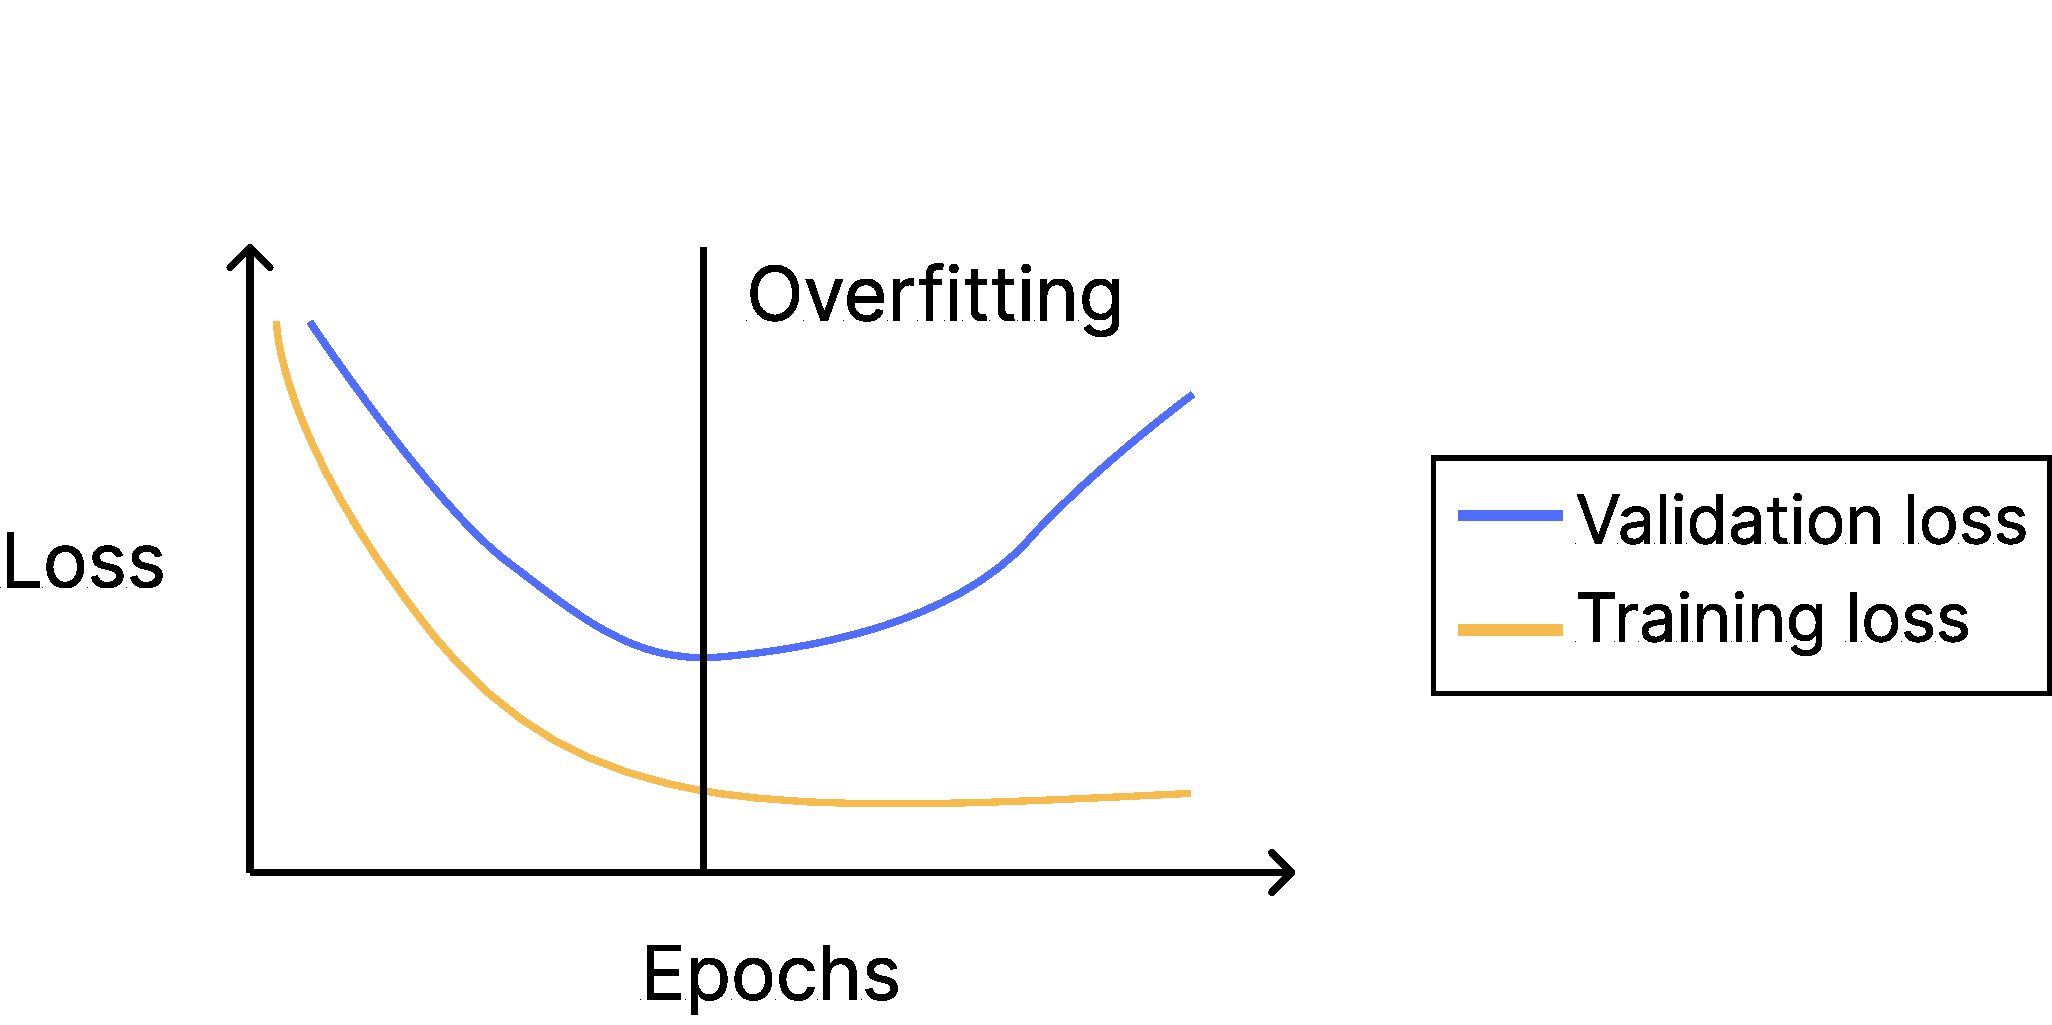
\includegraphics[width=0.6\textwidth]{obrazky-figures/overfitting.pdf}
	\caption[Overfitting illustrative graph]{An illustration of overfitting. Obtained from \cite{dataAugmentation1} and remade into PDF format for lossless scaling}
	\label{overfitting}
\end{figure}

Overfitting can be addressed by obtaining more training data. However, obtaining data for medical, niche, or generally difficult fields is not always a viable option. 

\textbf{Data augmentation} solves this problem by creating artificial/synthetic data. These can be created using traditional and deep learning/generative methods. This thesis focuses on traditional methods, such as changing the brightness or colors of the image. An example of this would be creating a copy of each data sample and decreasing its brightness, which may help the model perform better in dark conditions.


% ===========================================================================================

% ===========================================================================================

\section{Preprocessing}
\label{objectDetection}
Object detection, as a computer vision task, can be summarized in three steps: \textbf{preprocessing}, \textbf{inference}, and \textbf{postprocessing}. Where \textbf{preprocessing} is described in this section, followed by two sections describing \textbf{inference} and \textbf{postprocessing} processes, respectively.

The general knowledge about object detection was gained from Redmon's~\cite{Redmon_2016_CVPR} article on YOLO architecture. Further, more general knowledge on the overall process and training was gained from the YouTube tutorial series \cite{objectDetectioProcessYT_general, objectDetectioProcessYT_ultralitics} and Ultralytics' documentation and GitHub repositories \cite{ultralyticsGuide, ultralyticsRepo}

\begin{figure}[hbt]
	\centering
	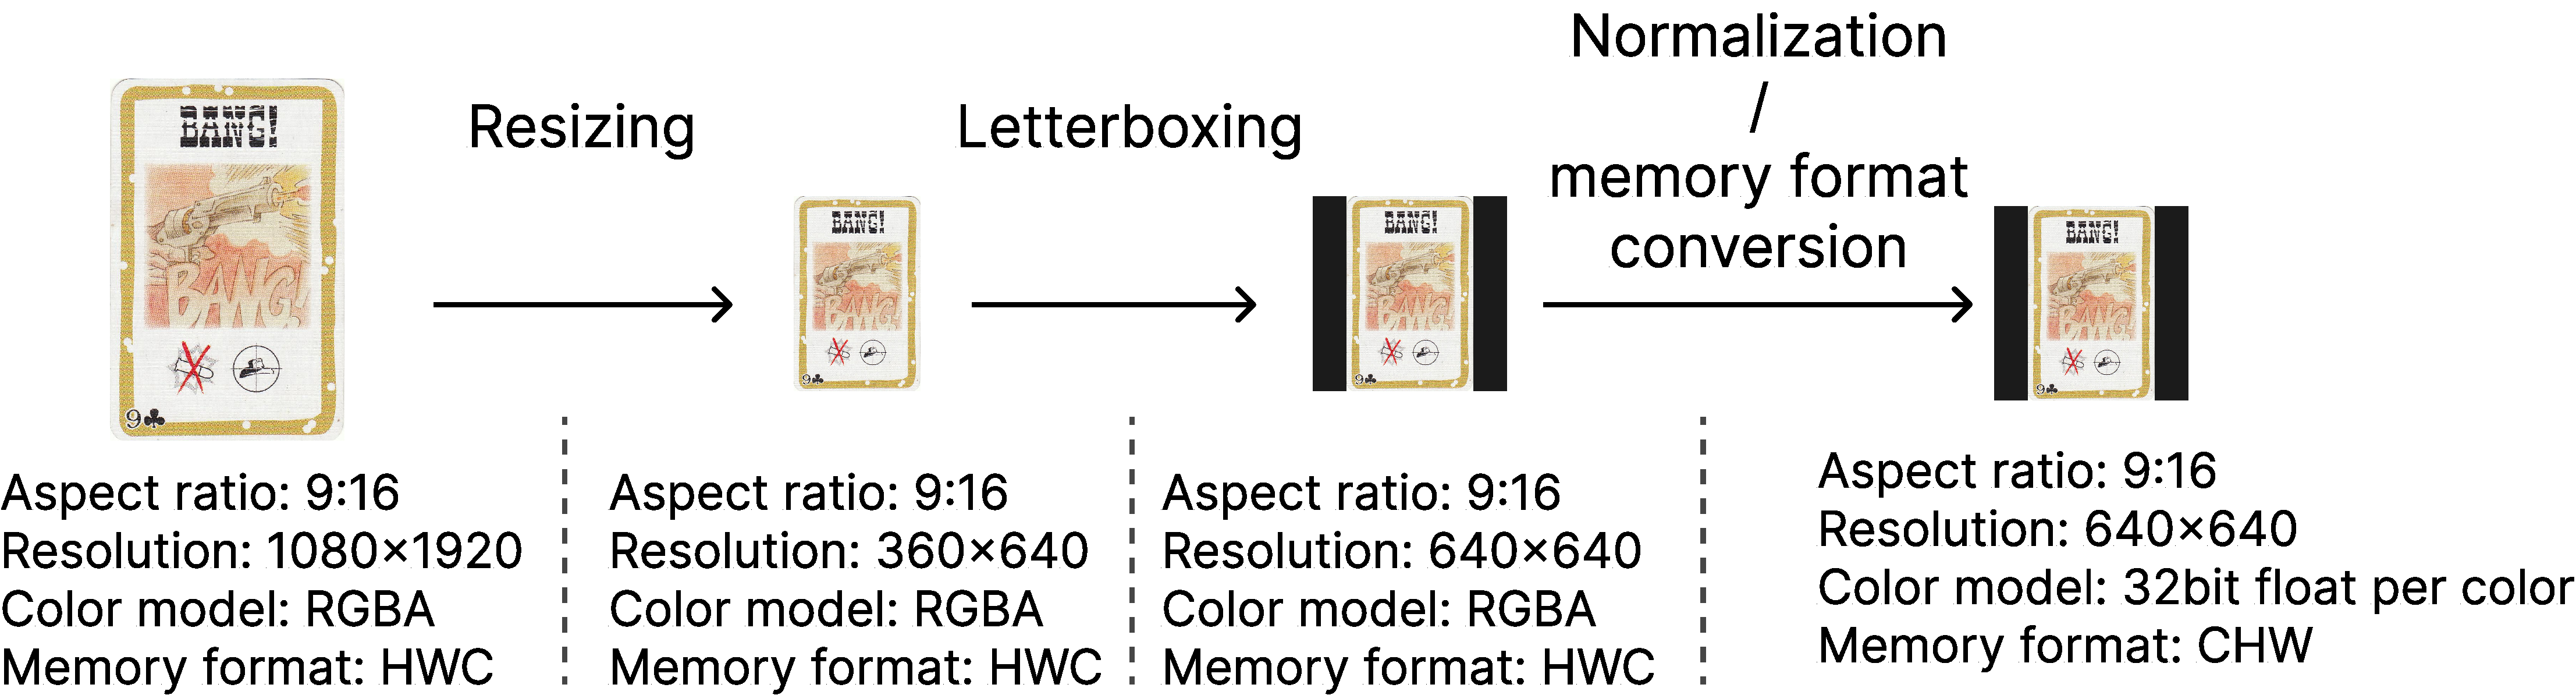
\includegraphics[width=1.0\textwidth]{obrazky-figures/preprocessing.pdf}
	\caption{Preprocessing steps shown on scan of the Bang! card from the game Bang!.}
	\label{preprocessingFigure}
\end{figure}


\label{imagePreprocessing}
Neural networks used for object detection are usually trained on preprocessed image data. Real world data are usually noisy, incomplete, inconsistent, and unbalanced. \textbf{Preprocessing} aims to clean these impurities and gives neural networks space to learn the important features needed for performing their tasks \cite{glossaryImagePreprocessing}. When passing image data into the neural networks, it is beneficial for the data to be preprocessed in the same way as it was during its training to achieve better results. 

\subsection{Letter-boxing and resizing}
\label{letterboxing}
Some object detection models need a fixed resolution in order to perform object detection tasks. However, the image data provided by the camera might not always be in the correct resolution, therefore, rescaling is needed \cite{letterboxingAndNormalization}.

For example, using a camera that provides a resolution of \texttt{1080x1920} in portrait mode, and the model, which requires an image with a resolution of \texttt{640x640}. Rescaling the image would create a \texttt{640x640} image; however, the original aspect ratio of the image was \texttt{9:16}. This would change to a \texttt{1:1} aspect ratio, and the distortion could affect object detection.

Instead, both dimensions will be scaled by the same scale factor, using the larger dimension, resulting in an image with a \texttt{640x360} resolution. However, this results in only one of the dimensions not satisfying the resolution required by the model. \textbf{Letter-boxing} fixes this problem by padding the image with a value/color in one of the dimensions. This will result in a final image not being distorted and in the correct \texttt{640x640} resolution.


\subsection{Normalization and representing colors in a image}
Images can be represented as a matrix or a 2-dimensional array of pixels, where each pixel is represented by three values: red, green, and blue. Most image formats use 8 bit or 16 bit unsigned integers for each color channel. This format is known as 8 bit or 16 bit RGB format, respectively. However, neural networks are mostly trained on normalized float values. Each color channel is converted into a float and normalized by the maximum value of the format; for 8 bit, this is \texttt{255}.

\subsection{Converting colors channel formats}
\label{hwcAndChwFormats}
The section above explained different ways of representing the values of each pixel in the image. However, the formats used to store these values in memory differ based on the needs of computer vision. Probably the most commonly used and intuitive way of storing image data is to use a 2-dimensional matrix of pixels, where each pixel is composed of three color values. This is called \textbf{HWC} format: Height x Width x Channel, where the channel refers to color values. For RGB format, there are three channels.

\begin{figure}[hbt]
	\centering
	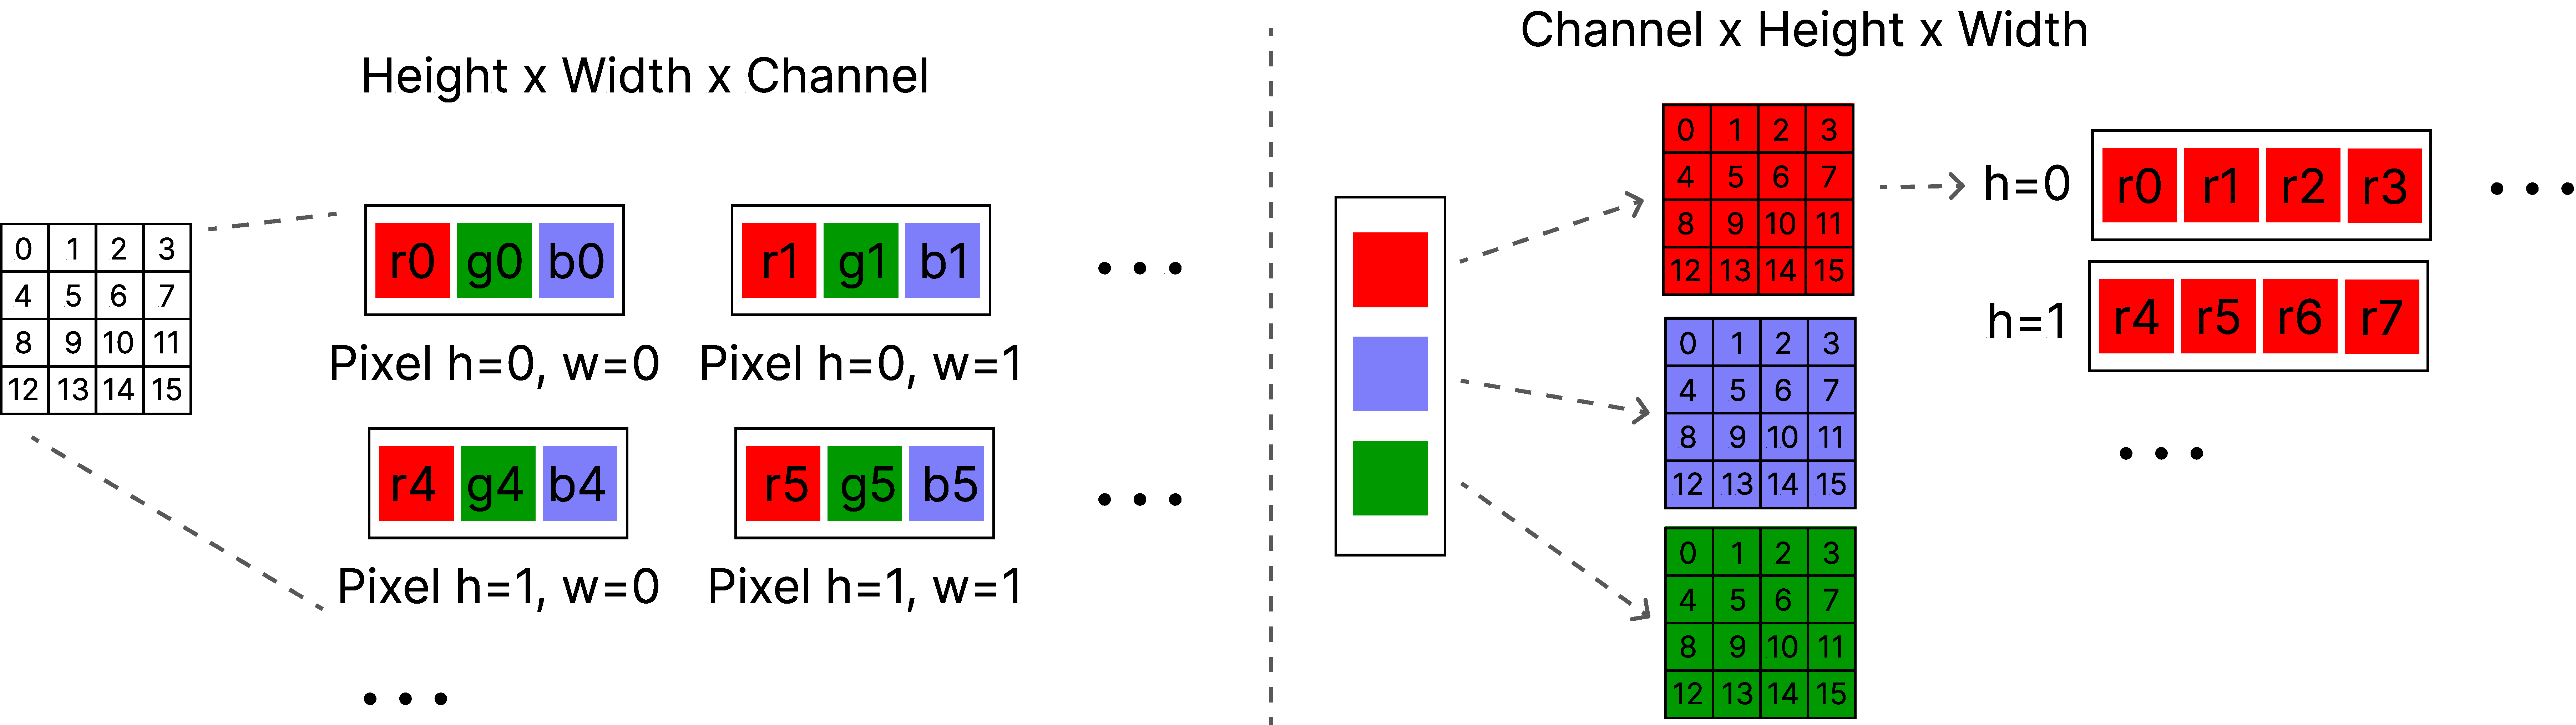
\includegraphics[width=1.0\textwidth]{obrazky-figures/channels.pdf}
	\caption[Image memory data layout of HWC and CHW]{Figure showing difference between HWC on the left, and CHW on the right. Both show 4x4 image with 3 color channels.}
	\label{ChannelsFigure}
\end{figure}

The commonly used format in neural networks, especially those aimed at image processing, is \textbf{CHW}. This format represents the image data in 3 sets of 2-dimensional matrices, each matrix containing values for a specific color, considering we are using RGB format with 3 color values \cite{channelFormatsSynopsis}. This format is beneficial for GPUs and NPUs as it is more suited for operations performed by these accelerators, especially parallel and vector operations \cite{chwAndHwcFormats}. 

A simple example of in-memory arrangement for these two formats for images with 3 color channels for a 2x2 image:

\begin{verbatim}
HWC
r0, g0, b0, r1, g1, b1, r2, g2, b2, r3, g3, b3

CHW
r0, r1, r2, r3, g0, g1, g2, g3, b0, b1, b2, b3
\end{verbatim}

Neural networks trained on data in \textbf{CHW} format will also expect this format during inference runs, meaning all image data used for object detection by the neural network must be converted to this format as well.

% ===============================

\section{Inference}
Inference in machine learning refers to the process of using a trained model to make predictions or decisions. This process applies the knowledge learned by the model and applies it onto new, unseen data, essentially solving real-world problems \cite{lenovoInference}. This task is performed by the \textbf{inference runtime}.

Neural networks are not executable by themselves and rely on dedicated inference engines or runtimes. Inference runtimes are responsible for executing trained neural network models by loading the model parameters, processing input data, and producing task-specific outputs. In this work, the runtime executes object detection using the deployed model to perform real-time object detection on image data.

% ===============================
\section{Postprocessing}
\label{postprocessing}
After preprocessing, the image was transformed into a suitable format usable by the neural network. The results of this inference run are further processed. This step is called \textbf{postprocessing}, and its purpose is to extract usually arrays of raw float values into a more structured data format.

\subsection{Data extraction}
\label{dataExtraction}
In order to extract values, it is necessary to know the layout of the data, which, for YOLO object detection models is: \texttt{[batch]x[attributes]x[detections]}. 

The \textbf{batch} value in this project is always 1 because the implemented object detection algorithms are meant for realtime processing and always use only a single image as input. Therefore, the shape is effectively \texttt{[attributes]x[detections]}. 

The \textbf{attributes} are individual values that depend on the used model. For the object detection models, these values are usually: coordinates describing the bounding box of the detection and confidence scores. Bounding boxes are 2-dimensional representations of detected objects. Confidence score values are a representation of how confident the model is for the current class. An example showing outputs from the YOLO version 8 and 26:
\begin{verbatim}
    Output of the YOLO 8:
    x, y, width, height, class 0 confidence, class 1 confidence, ...
    Output of the YOLO 26:
    x, y, width, height, best class, confidence score
\end{verbatim}

\textbf{Detections} refer to the number of detections found by the model. For the YOLOv8 models, this value represents grid like feature maps: 80x80 + 40x40 + 20x20 = 8400\footnote{How YOLOv8 Works: \url{https://nvidia-isaac-ros.github.io/concepts/object_detection/yolov8/index.html\#how-yolov8-works}}.

\begin{figure}[hbt]
	\centering
	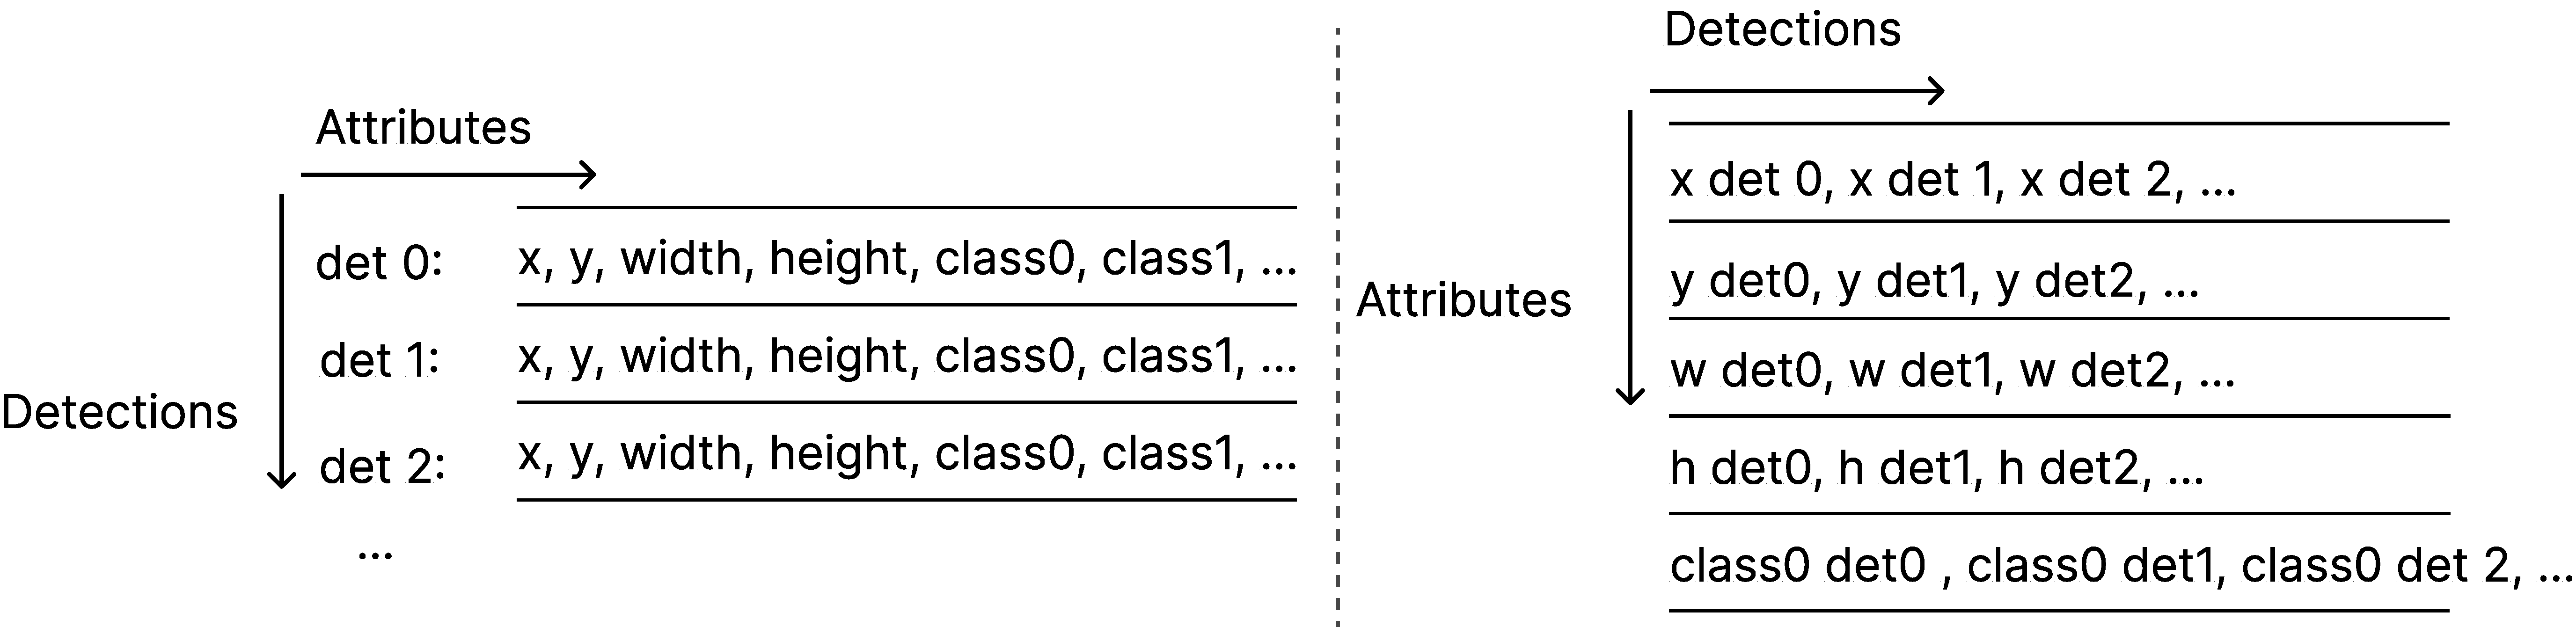
\includegraphics[width=0.98\textwidth]{obrazky-figures/extracted_data_layout.pdf}
	\caption[Memory layout of raw extracted detections]{Figure showing data layout in memory, on the left [detections]x[attributes], on the right [attributes]x[detections].}
	\label{ExtractedDataLayoutFigure}
\end{figure}

\subsection{Reading data}
\label{readingDataFormats}
Outputs of the object detection models are in \texttt{[attributes]x[detections]} shape, which might not be the most intuitive one. Therefore, there are two options: use it as it is or transpose the data. Both are valid options, and in mathematics, transposing might be preferred. However, performing these operations on already resource limited devices is not an optimal solution.

\begin{verbatim}
    // data : array containing data in [attributes]x[detections] format 
    for (column in 0 until numberOfDetections) {
        val x = data[0 * numberOfDetection + column]
        val y = data[1 * numberOfDetection + column]
        // ...
    }    
\end{verbatim}

\begin{verbatim}
    // data : array containing data in [detections]x[attributes] format 
    for (attributes in data) {
        val x = attributes[0]
        val y = attributes[1]
        // ...
    }    
\end{verbatim}

The abstract code snippet above shows the difference between the two approaches. A very simple test for both of these methods shows that transposing the data is 3 times slower (approximately \texttt{5.18 milliseconds}) for YOLO 8, with its 8400 detections. Therefore, a direct approach mirroring the memory layout used in this project.

\subsection{Thresholding}
Thresholding, or confidence score filtering, is a simple process for removing \textbf{detections} whose confidence score is below the threshold. Due to their architecture, object detection models tend to produce a lot of low confidence predictions; more specifically, they produce predictions for each region and choose the most probable class. Therefore, it is necessary to remove these extra detections.

\subsection{Non-Maximum Suppression}
The object detection model might output multiple bounding boxes for one object. These duplications need to be removed, and the most proven method is \textbf{Non-Maximum Suppression} \cite{nms}. If the computed \textbf{Intersection Over Union} or \textbf{IoU} for two detections is past a threshold, the detection with the lower confidence score is removed. The NMS algorithm can be simplified into 3 steps \cite{nms}:

\begin{enumerate}
  \item {Choose the detection with the highest confidence score from all detections, remove it from the list of all detections, and add it to the list of kept ones.}
  
  \item {Compute IoU for the chosen detection, from the 1st step, and the rest of the detections. If the IoU is above the threshold, remove the detection with lower confidence score from the list of all detections.}
  
  \item {Repeat until the list of all detections is empty.}
\end{enumerate}

Non-Maximum suppression, as it is, can result in objects of different classes removing one another. For example, an apple held in a human hand is being deleted because it overlaps with a human who has a higher confidence score. To help solve this problem, NMS is applied only to the same classes; therefore, only the human class can remove another human class.

\begin{figure}[hbt]
	\centering
	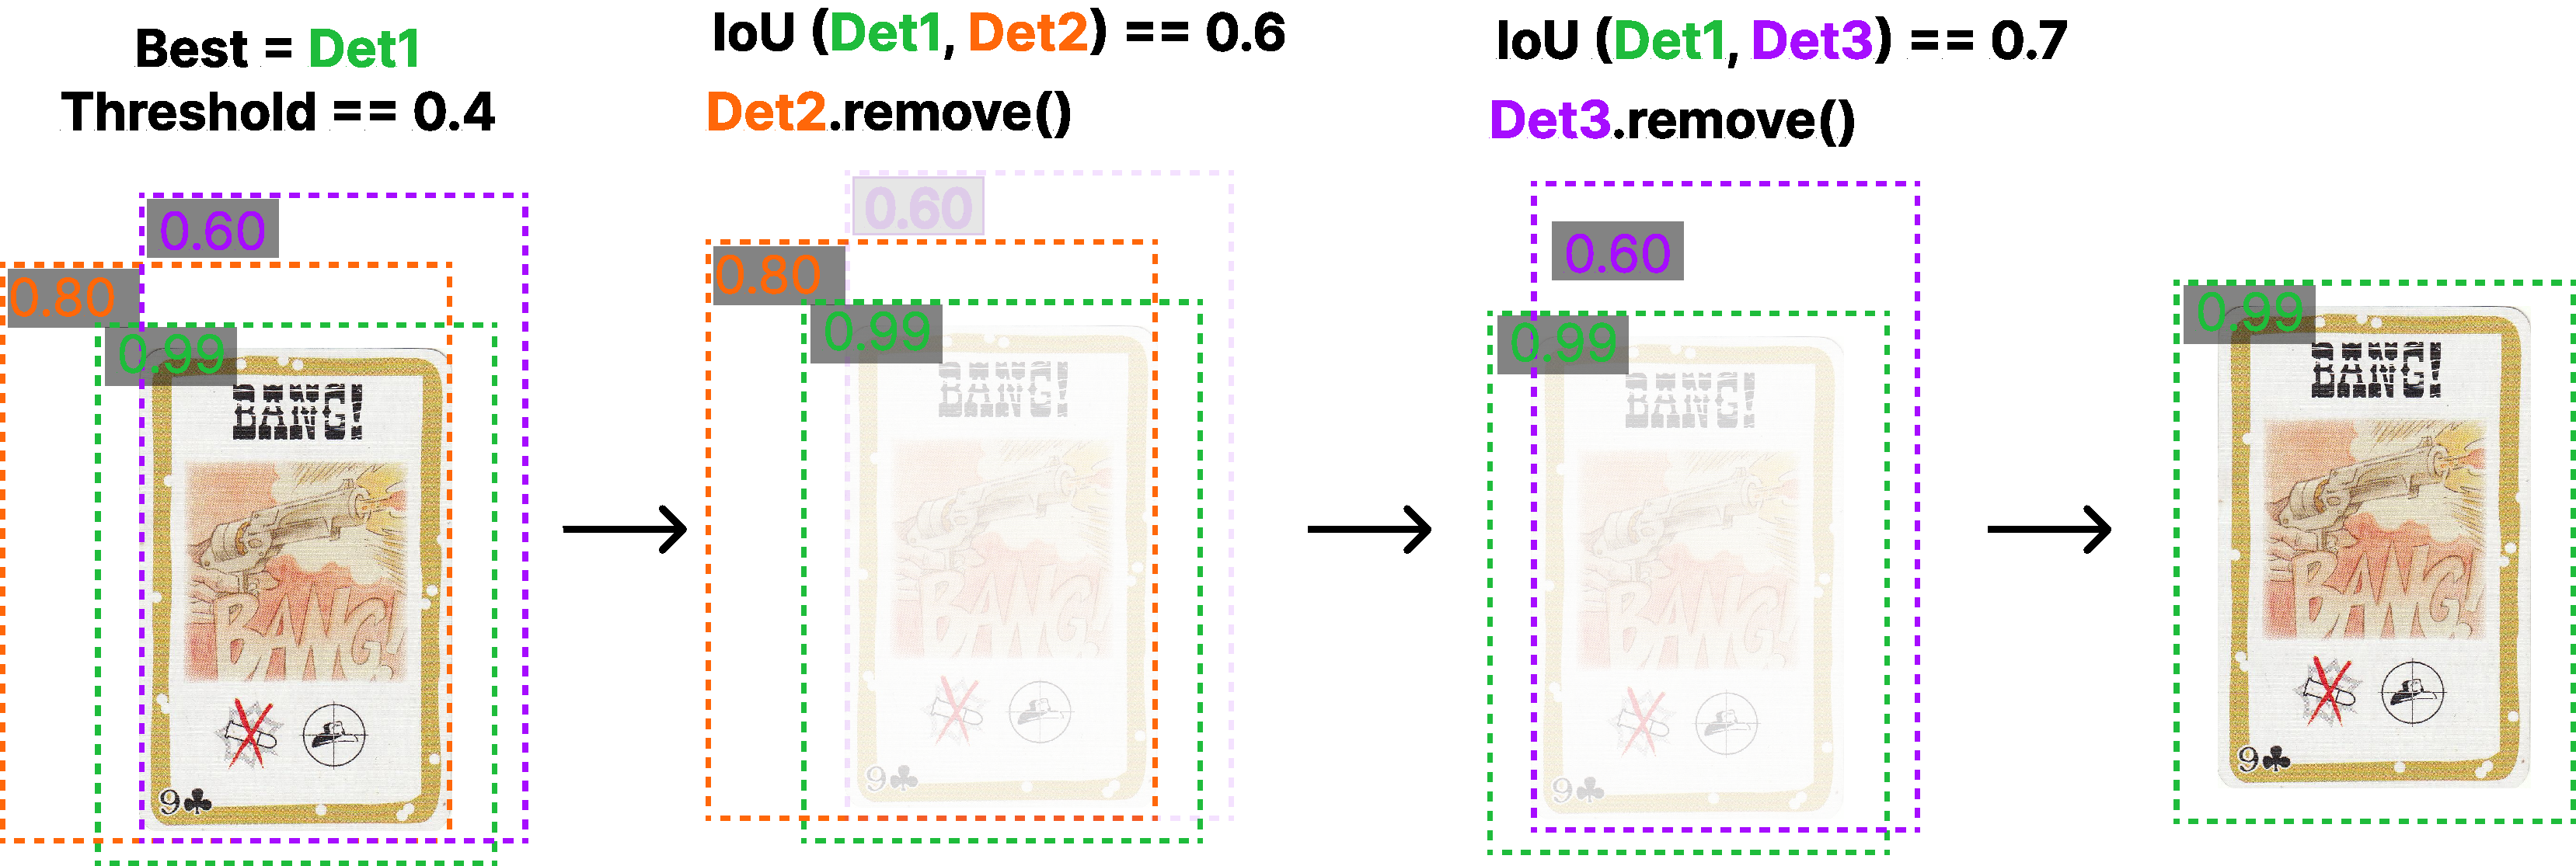
\includegraphics[width=0.80\textwidth]{obrazky-figures/nms_example.pdf}
	\caption{Simplified Non-Maximum Suppression demonstration.}
	\label{nsmDemonstration}
\end{figure}

NMS is not a cheap operation, especially with many objects in one scene, as it has to iterate through all detected objects multiple times. Therefore, it is recommended to first reduce the number of detections using thresholding or other methods \cite{nms}. Lastly, NMS can use confidence softening instead of removing detections. However, this approach was implemented for real-time detection tasks as it would require multiple repetitions. 